\documentclass[conference]{IEEEtran}
\IEEEoverridecommandlockouts
\usepackage{cite}
\usepackage{amsmath,amssymb}
\usepackage{graphicx}
\usepackage{url}
\usepackage{array}
\usepackage[T1]{fontenc}
\usepackage{booktabs}
\newcolumntype{L}[1]{>{\raggedright\arraybackslash}p{#1}}
\newcolumntype{C}[1]{>{\centering\arraybackslash}p{#1}}
\graphicspath{{figures/}}
\hyphenpenalty=200 \tolerance=1200 \emergencystretch=1.5em

\begin{document}

\title{Quantifying the Incremental Value of\\ Retrieval-Side Reliability Signals for\\ Selective Extractive Question Answering}

\author{%
\IEEEauthorblockN{Harsh Kamat, Harsh Ranjan, Manish Kumar, Divya Tyagi, and Snigdha Kesh}
\IEEEauthorblockA{\textit{Department of Computer Science and Engineering}\\
\textit{AMC Engineering College, Visvesvaraya Technological University}\\
Bengaluru, India}%
\thanks{H. Kamat, H. Ranjan and M. Kumar performed the implementation and
experiments. D. Tyagi supervised the work as project guide. S. Kesh served as
project coordinator. Institutional e-mail addresses and ORCID identifiers are
omitted pending confirmation.}%
}

\maketitle

\begin{abstract}
A question-answering system that never declines will eventually present a
fabricated span with the same confidence as a correct one. Training a classifier
to anticipate reader errors is an established remedy, but it was formulated
without a retrieval stage, and later retrieval-aware variants assume a large
generative model. How much error-prediction information the retrieval stage
itself contributes, once a reader-side calibrator is already fitted, has not been
isolated for pipelines that cannot afford a second model pass. We measure that
increment. Our system runs entirely on a CPU with no pretrained neural weights:
latent-semantic and BM25 retrieval, a two-stage feature-based span reader with a
learned no-answer head, sixteen reliability signals drawn from retrieval, reading
and cross-passage agreement, a gradient-boosted risk estimator, and isotonic
calibration. Evaluated on 3{,}585 questions from 36 withheld SQuAD 2.0 articles
with article-level partitioning, a shuffled-label control returns an
error-prediction ROC-AUC of 0.4887 inside its pre-registered 0.45--0.55 band. The
combined signal set reaches an error-prediction ROC-AUC of 0.6390 (95\% bootstrap
interval 0.6127--0.6668) where a reader-only calibrator reaches 0.5242, and
reduces the area under the risk--coverage curve by 0.0345 (paired 95\% bootstrap
interval for $\Delta$AURC $= [-0.0495,-0.0191]$, excluding zero); the ordering is
unchanged at correctness cut-offs
of 0.4, 0.5 and 0.6. Withholding feature families implicates retrieval most
clearly ($\Delta$AURC 0.0274) and agreement next (0.0103), while withholding all
five reader signals leaves an interval spanning zero (0.0067). The added layer
costs 1.96\,ms of a 63.77\,ms query. These findings are bounded by a deliberately
simple reader: base accuracy is 0.1144 and three of seven pre-registered gates
failed. We claim the measurement, not the mechanism.
\end{abstract}

\begin{IEEEkeywords}
selective prediction, question answering, abstention, confidence calibration,
uncertainty estimation, information retrieval, resource-constrained inference
\end{IEEEkeywords}

\section{Introduction}
Silence is not a failure mode that document question-answering systems support
well. Given a query whose answer is absent from the collection, a retrieval-based
reader still emits a span, still attaches it to a genuine passage, and still
formats it exactly as it would format a correct response. Nothing in the output
separates the two cases, so a cautious user must check every answer, which erases
the reason for deploying the system.

Deciding whether to publish an extracted span is therefore a separate problem from
extracting it. The reader's own probability is a poor instrument for that decision.
It is normalised over candidate spans inside a passage that was handed to the
reader, so it can express which span is locally best but not whether the passage
deserved to be retrieved. Two situations are consequently invisible to it: the
collection holds no answer, and the retriever ranked the relevant passage out of
reach. Together these describe 29.5\% and 6.1\% of our evaluation set.

Statistics produced during retrieval do see that region, and they cost nothing
extra. Similarity values, the gap between competing passages and the shape of the
score distribution are already computed before the reader begins. Whether
independently retrieved passages converge on the same string is equally cheap.

None of this is a new observation. Selective prediction rests on established
theory \cite{elyaniv2010,geifman2017}; error-predicting calibrators for question
answering were introduced by Kamath, Jia and Liang \cite{kamath2020}; reading
calibration at scale was examined by Dhuliawala \emph{et al.} \cite{dhuliawala2022};
and the sufficiency of retrieved context has been studied from several directions
\cite{joren2025,abdumalikov2024,lewis2021,muhamed2025}. \textbf{We make no claim to
have introduced retrieval-aware abstention.}

The quantity that remains unmeasured is the increment. Holding fixed a reader-side
calibrator of the type established in \cite{kamath2020}, how much further
error-prediction information do retrieval and cross-passage signals supply under
matched partitions and interval estimation? And does that increment persist once
the pipeline is restricted to a CPU with no pretrained weights, the regime where
the low cost of these signals matters most? This paper reports both measurements.

\noindent\textbf{Contributions.}
\begin{enumerate}\itemsep0.5pt
\item A controlled procedure for separating the reliability information carried by
retrieval, reader and agreement signals, built on article-level partitions, a
shuffled-label control and article-clustered bootstrap intervals.
\item A sixteen-signal reliability representation derived solely from quantities
the pipeline has already computed, adding no inference pass.
\item A comparison against five alternatives: unconditional answering, two
single-signal thresholds, the reader's own no-answer head, and a reader-only
calibrator reproducing \cite{kamath2020} in our pipeline.
\item Family-withholding ablation with a permutation cross-check, a transfer
evaluation on a disjoint collection, an outcome taxonomy, and per-stage cost
measurement.
\item Evidence that the combined representation sharpens error discrimination and
lowers selective risk against the reader-only calibrator in this CPU-only setting,
reported alongside the pre-registered criteria it did not meet.
\end{enumerate}

\section{Related Work}
\textbf{Selective prediction.} Pairing a predictor with a gate that may withhold a
decision was formalised by El-Yaniv and Wiener \cite{elyaniv2010} and carried to
deep models by Geifman and El-Yaniv \cite{geifman2017}. Performance is summarised
by the risk--coverage curve, whose area (AURC) we adopt as the primary quantity.
Smaller values indicate better selective behaviour.

\textbf{Calibration.} Guo \emph{et al.} \cite{guo2017} documented that modern
classifiers report unreliable confidence and compared post-hoc corrections.
Isotonic regression as a calibration map originates with Zadrozny and Elkan
\cite{zadrozny2002}. We use it and report expected calibration error (ECE) on
either side of the correction.

\textbf{Error prediction in reading systems.} Kamath, Jia and Liang
\cite{kamath2020} demonstrated that a classifier trained to anticipate reader
mistakes outperforms thresholding the reader's softmax, most visibly under domain
shift. Because their reader receives a designated passage, retrieval-derived
signals fall outside their formulation. We reproduce their approach over our
reader's outputs as baseline B5 and treat it as the target to beat rather than a
convenient foil. Dhuliawala \emph{et al.} \cite{dhuliawala2022} reached a
compatible conclusion at larger scale. The unanswerable questions of SQuAD 2.0
\cite{rajpurkar2018} are what make abstention measurable at all.

\textbf{Sufficiency of retrieved context.} Joren \emph{et al.} \cite{joren2025}
define \emph{sufficient context} and observe that capable models frequently answer
when the retrieved material cannot support an answer, proposing sufficiency-guided
selective generation. Abdumalikov \emph{et al.} \cite{abdumalikov2024} report that
rejection models trained against randomly paired passages transfer poorly to
distractors sharing vocabulary with the query, accuracy collapsing from 98\% to
1\%, and repair this using SQuAD 2.0 unanswerable pairs. Muhamed \emph{et al.}
\cite{muhamed2025} perturb grounding material systematically and find refusal
accuracy under 50\% on multi-document inputs, further separating refusal into
detection and categorisation abilities. Lewis \emph{et al.} \cite{lewis2021} show
that retrieval scores alone permit selective answering along a tunable
accuracy--coverage curve.

\textbf{Positioning.} Collectively this work establishes the theory of selective
prediction, the advantage of trained error predictors over raw reader confidence,
and the diagnostic value of context sufficiency. It does not isolate the
\emph{marginal} contribution of retrieval and agreement signals \emph{given} a
reader-side calibrator in a pipeline barred from a second large-model pass. The
nearest studies \cite{joren2025,muhamed2025,lewis2021} operate with large
generative models or large neural retrievers. \emph{We claim the measurement, not
the mechanism.}

\section{Problem Formulation and Scope}
\textbf{Question.} Do retrieval-side and cross-evidence reliability signals supply
incremental error-prediction value beyond a reader-only calibrator in a CPU-only
extractive question-answering pipeline?

Secondary questions concern whether reader error is predictable at all here,
whether the combination surpasses the reader's own no-answer head, whether the
resulting estimate is calibrated, which family is responsible, whether the
estimator transfers to an unseen collection, and what it costs.

\textbf{Formulation.} For a query $q$, a collection $C$, a retrieved subset
$R \subseteq C$ and an extracted span $\hat{a}$, we require
$g(q,R,\hat{a}) \rightarrow [0,1]$ approximating $P(\hat{a}\ \text{is wrong})$,
together with a cut-off $\tau$ such that responding only when $g < \tau$ realises a
chosen operating point.

\textbf{Correctness.} An answerable query counts as handled correctly when the
returned span attains SQuAD F1 $\geq 0.5$ against any reference; an unanswerable
query counts as handled correctly only when nothing is returned. The prediction
target is the complement. SQuAD normalisation precedes scoring. The framing assumes
an incorrect answer is more costly than silence, which is a property of the
deployment rather than something we establish.

\section{Data and Protocol}
\subsection{Answerability once retrieval is introduced}
The SQuAD 2.0 label is defined against a single paragraph: a query marked
unanswerable was unanswerable \emph{from the paragraph shown to the annotator}.
Retrieval dissolves that guarantee. Once other paragraphs enter the collection an
``unanswerable'' query may become answerable, and the label quietly ceases to
describe what is being scored.

We sized the exposure before fixing the design. Each unanswerable SQuAD 2.0 item
carries a \texttt{plausible\_answer}: the most persuasive incorrect span from its
own paragraph. Occurrence of that string elsewhere in the collection is a concrete
path to an invalid label. Counting over 40 randomly drawn training articles, and
restricting attention to substantive strings ($\geq 2$ tokens, not purely numeric,
$\geq 6$ characters, $n = 3{,}049$), \textbf{14.89\%} of such strings reappear when
an article's own sibling paragraphs are pooled into the collection, against
\textbf{2.39\%} when they are excluded --- a sixfold reduction.

Roughly one substantive unanswerable label in seven would therefore be
compromised by pooling, which exceeds any effect we intend to detect. We adopt the
\textbf{sibling-masked} arrangement: a query may reach its own source paragraph and
any paragraph from a \emph{different} article, never another paragraph of its own
article.

Answerable labels survive because the source paragraph always remains reachable;
failure to rank it inside the top-$k$ is then a real retrieval error of the kind
under study. Unanswerable labels survive because the only same-topic paragraph in
scope is the one against which the annotator judged the query unanswerable. Masking
consults the article identifier alone and is applied uniformly to both classes;
conditioning it on the label would import the target into the collection. The
construction is the familiar distractor arrangement from multi-document QA, used
here to protect labels rather than to raise difficulty.

Paragraphs enter whole. A median SQuAD paragraph is 107 tokens, inside the reader's
span window, so we do not sub-divide; doing so would cut reference spans at
boundaries and add a confound unrelated to the question.

\subsection{Collections and partitions}
Collection~A supplies the main experiment: 120 articles sampled from SQuAD 2.0
train, 5{,}637 paragraphs, 11{,}921 queries, 31.17\% unanswerable. Collection~B is
the complete SQuAD 2.0 development set, reserved for transfer: 35 articles, 1{,}204
paragraphs, 3{,}500 queries, 50.46\% unanswerable. Their article titles do not
intersect.

Partitions are cut \textbf{by article}. SQuAD supplies a median of 279 queries per
article, many revisiting the same facts, so dividing at the query level scatters
near-duplicates across both sides and inflates every estimate. Three partitions do
not suffice, because two models are fitted: a reliability estimator trained on
articles the reader has already absorbed would observe an error distribution far
more favourable than the one it meets at test time. Collection~A is therefore split
40/20/10/30 by article into \texttt{reader\_train} (48 articles),
\texttt{rel\_train} (24 articles, 2{,}400 queries), \texttt{rel\_calib} (12
articles, 1{,}200 queries) and \texttt{test} (36 articles, 3{,}585 queries).
Disjointness is asserted by a unit test that fails the build.

\subsection{Pre-registration and interval estimation}
Seven numeric criteria were recorded before execution and none was revised
afterwards. Every run uses seed 20260814; hyperparameters remain at library
defaults and were never tuned against the test partition. Intervals come from a
cluster bootstrap over \textbf{articles} with 1{,}000 resamples, since queries
within an article are dependent and resampling queries would understate the spread.
Two-method comparisons use a paired bootstrap over identical article resamples.

\begin{figure}[!t]
\centering\scriptsize
\setlength{\fboxsep}{3.5pt}
\framebox[\columnwidth][l]{%
\begin{minipage}{0.93\columnwidth}
\ttfamily
query\\
\quad$\downarrow$ \textbf{RETRIEVAL} \ TF-IDF $\rightarrow$ SVD(256) $\rightarrow$ inner product\\
\quad\phantom{$\downarrow$ } BM25Okapi; fuse $\alpha{=}0.5$; sibling mask\\
\quad$\downarrow$ top-$k$ paragraphs + scores\\
\quad\phantom{$\downarrow$ }\textbf{READER} \ 1. keep 3 best-matching sentences\\
\quad\phantom{$\downarrow$ } 2. $n$-grams $\leq 8$, drop stopword/punct edges\\
\quad\phantom{$\downarrow$ } 3. GBM span scorer (20 span features)\\
\quad\phantom{$\downarrow$ } 4. GBM no-answer head $\rightarrow$ P(no answer)\\
\quad$\downarrow$ span, span prob., no-answer score, entropy\\
\quad\phantom{$\downarrow$ }\textbf{RELIABILITY LAYER (measured)}\\
\quad\phantom{$\downarrow$ } retrieval(7) + reader(5) + agreement(4)\\
\quad\phantom{$\downarrow$ } GBM $\rightarrow$ isotonic $\rightarrow$ P(error)\\
\quad$\downarrow$\\
risk $>\tau$ ? \ yes $\rightarrow$ abstain + reason\\
\phantom{risk $>\tau$ ? \ }no \ $\rightarrow$ answer + paragraph + risk
\end{minipage}}
\caption{Pipeline. Every block was implemented and exercised in the reported
experiments; the cut-off $\tau$ is fixed on the calibration partition only.}
\label{fig:arch}
\end{figure}

\section{System}
\subsection{Retrieval}
Paragraphs become TF-IDF vectors compressed to 256 dimensions by truncated SVD ---
latent semantic analysis in the sense of Deerwester \emph{et al.}
\cite{deerwester1990} --- and are searched exactly by inner product. A BM25Okapi
index \cite{robertson2009} operates alongside. Both score vectors are min--max
scaled across the candidate set and averaged with equal weight. The compressed
representation absorbs paraphrase; the lexical index restores exact names, figures
and identifiers that a 256-dimensional projection dilutes, and yields the
query--paragraph overlap statistic that later proves the most load-bearing
reliability signal.

\subsection{Reader}
The first stage orders a paragraph's sentences by overlap with the query's content
words and retains three. Measured on training articles, 68.2\% of reference answers
occur in the single best sentence and 83.3\% within the best three, so the
candidate space contracts sharply at modest cost. The second stage enumerates token
$n$-grams up to length eight inside those sentences, removes any span whose first
or last token is a stopword or punctuation --- a filter that preserves 90.4\% of
reference answers while discarding 64\% of candidates --- and scores what remains
with a gradient-boosted classifier over twenty span descriptors covering
capitalisation, numerals, inverse document frequency, proximity to query terms,
sentence overlap, surrounding context and interactions with the interrogative type.
A second gradient-boosted model, fitted on the same articles against the
\texttt{is\_impossible} flag, emits $P(\text{this paragraph holds no answer})$. The
reader thus presents the same interface as a transformer trained on SQuAD 2.0 --- a
best span, a span score, an explicit no-answer score --- without pretrained weights.

\textbf{Constraint.} A DistilBERT reader and MiniLM embeddings were specified
originally. Neither could be retrieved: every route to the model repository was
blocked in our build environment. Rather than fabricate numbers or abandon the
study, we substituted established methods needing no pretrained weights while
preserving the interface the question depends on. \textbf{No transformer, learned
embedding or pretrained language model appears anywhere in the evaluated system.}
Section~\ref{sec:lim} quantifies what this costs.

\subsection{Reliability signals and the gate}
Sixteen signals in three families (Table~\ref{tab:feats}), each read from
quantities the pipeline has already produced. A gradient-boosted classifier maps
them to a risk score; isotonic regression \cite{zadrozny2002} fitted on the
calibration partition converts that score into an estimated error probability; a
cut-off is then chosen on the same partition.

\begin{table}[!t]
\renewcommand{\arraystretch}{1.15}
\caption{The sixteen reliability signals.}
\label{tab:feats}
\centering\footnotesize
\begin{tabular}{L{1.45cm}L{6.0cm}}
\toprule
\textbf{Family} & \textbf{Signals} \\
\midrule
Retrieval (7) & best fused score; separation between the two best; mean over
top-$k$; entropy of the score distribution over a wider list; count exceeding a
similarity floor; query--paragraph lexical overlap; query length \\
\addlinespace[1.5pt]
Reader (5) & span probability; no-answer score; their difference; span length;
entropy of the span score distribution \\
\addlinespace[1.5pt]
Agreement (4) & paragraphs among the top-$k$ yielding a non-empty span; edit
similarity between the two leading spans; share of top-$k$ spans equal to the modal
span; whether the selected span recurs in the second paragraph \\
\bottomrule
\end{tabular}
\end{table}

Two points require care. \textbf{Isotonic regression aligns the score with observed
error frequency; it certifies nothing.} The system estimates risk and applies a
cut-off, and Section~\ref{sec:calib} records an operating point it failed to
realise. Second, no signal triggers an additional model pass, which is what holds
the layer at 1.96\,ms instead of doubling inference, and why richer signals
available in the literature were excluded deliberately.

\section{Baselines and Ablation Design}
The six procedures in Table~\ref{tab:methods} consume identical pipeline output over
identical partitions; only the signal driving the decision differs. \textbf{The
comparison that answers the question is P1 against B5}, not P1 against B1.

\begin{table}[!t]
\renewcommand{\arraystretch}{1.15}
\caption{Decision procedures compared.}
\label{tab:methods}
\centering\footnotesize
\begin{tabular}{L{0.45cm}L{3.3cm}L{3.3cm}}
\toprule
\textbf{ID} & \textbf{Procedure} & \textbf{Signal} \\
\midrule
B1 & Answer unconditionally & none (floor) \\
B2 & Span-probability cut-off & reader softmax \\
B3 & Retrieval-score cut-off & best fused score \\
B4 & Reader no-answer head & the reader's own trained head \\
B5 & Reader-only calibrator, after \cite{kamath2020} & the 5 reader signals \\
P1 & Combined calibrator (evaluated) & all 16 signals \\
\bottomrule
\end{tabular}
\end{table}

The ablation withholds one family at a time and additionally fits each family
alone --- seven configurations settled in advance. Permutation importance over the
full model supplies an independent attribution. A shuffled-label control runs
first; unless it returns to chance, no downstream figure is reported.

\section{Results}\label{sec:results}
\subsection{Control}
Permuting the error labels and refitting yields an error-prediction ROC-AUC of
\textbf{0.4887} on the test partition, inside the pre-registered band
$[0.45,0.55]$. Criterion G0 is met; no leakage is detectable through the signals,
the partitions or the calibration step.

\subsection{Main comparison}
Table~\ref{tab:main} gives all six procedures. P1 leads throughout, and its interval
is disjoint from those of B2, B4 and B5.

\begin{table*}[!t]
\renewcommand{\arraystretch}{1.2}
\caption{Selective prediction over 3{,}585 test queries from 36 withheld articles.
Intervals are 95\% cluster bootstrap over articles. Lower AURC is better.
SelAcc@$c$ denotes selective accuracy at coverage $c$.}
\label{tab:main}
\centering\footnotesize
\begin{tabular}{L{4.3cm}C{1.9cm}C{2.2cm}C{1.6cm}C{2.2cm}C{1.5cm}C{1.5cm}}
\toprule
\textbf{Procedure} & \textbf{Error ROC-AUC} & \textbf{95\% interval} &
\textbf{AURC} & \textbf{95\% interval} & \textbf{SelAcc@0.5} & \textbf{SelAcc@0.7} \\
\midrule
B1 \ answer unconditionally        & 0.5000 & ---            & 0.8890 & 0.8455--0.9162 & 0.0988 & 0.1064 \\
B2 \ span probability              & 0.4920 & 0.4544--0.5304 & 0.8823 & 0.8498--0.9084 & 0.1066 & 0.1143 \\
B3 \ retrieval score               & 0.5634 & 0.5353--0.5925 & 0.8686 & 0.8362--0.8962 & 0.1328 & 0.1263 \\
B4 \ reader no-answer head         & 0.5526 & 0.5216--0.5823 & 0.8683 & 0.8365--0.8982 & 0.1267 & 0.1235 \\
B5 \ reader-only calibrator \cite{kamath2020} & 0.5242 & 0.5080--0.5428 & 0.8785 & 0.8412--0.9019 & 0.1071 & 0.1112 \\
\textbf{P1 \ combined (evaluated)} & \textbf{0.6390} & \textbf{0.6127--0.6668} & \textbf{0.8423} & \textbf{0.8029--0.8731} & \textbf{0.1462} & \textbf{0.1355} \\
\bottomrule
\end{tabular}
\end{table*}

Two entries deserve emphasis. B2 --- a cut-off on reader confidence, the reflexive
choice in practice --- produces an interval straddling 0.5 and is thus not
separable from chance here. And the two retrieval-aware single signals, B3 (0.5634)
and B4 (0.5526), both exceed the reader-only \emph{calibrator} B5 (0.5242), despite
B5 combining five signals through a fitted model.

\subsection{The increment}
Paired bootstrap over articles, identical resamples for both procedures:
\begin{itemize}\itemsep0.5pt
\item $\Delta$AURC (P1 $-$ B5) $= -0.0345$, 95\% interval $[-0.0495,-0.0191]$,
excluding zero. P1 \emph{reduces} AURC relative to B5. Criterion G3 is met.
\item $\Delta$AURC (P1 $-$ B4) $= -0.0293$, 95\% interval $[-0.0442,-0.0150]$,
excluding zero. Criterion G4 is met.
\end{itemize}
These are paired-bootstrap intervals excluding zero. No null-hypothesis test was
performed and we do not describe the outcome as statistically significant.

The 0.5 correctness cut-off is a choice, so the comparison was repeated at 0.4 and
0.6. P1 reaches an error-prediction ROC-AUC of 0.6431 and 0.6352 against 0.5132 and
0.5354 for B5, with $\Delta$AURC of $-0.0438$ $[-0.0633,-0.0263]$ and $-0.0294$
$[-0.0445,-0.0169]$. Direction and interval behaviour are unaffected by the cut-off.

\begin{figure}[!t]
\centering
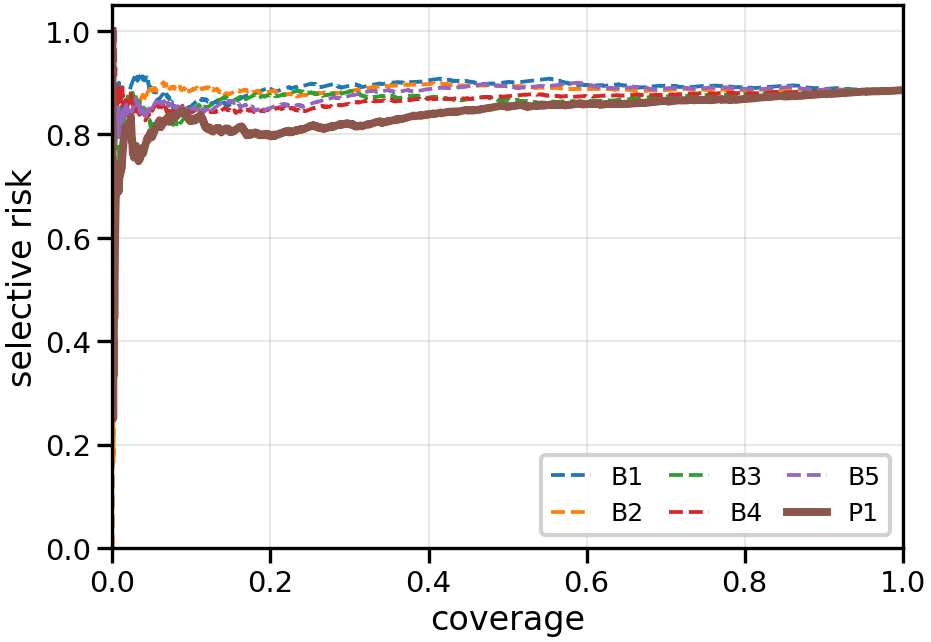
\includegraphics[width=\columnwidth]{F3_risk_coverage.png}
\caption{Risk--coverage behaviour of all six procedures on the test partition.
Lower curves indicate lower selective risk; P1 generally lies below the baselines
across the coverage range.}
\label{fig:rc}
\end{figure}

\subsection{Calibration and an operating point that was not reached}\label{sec:calib}
Isotonic regression lowers expected calibration error from \textbf{0.0895 to
0.0120}, inside the 0.10 criterion, and Fig.~\ref{fig:cal} shows the corresponding
movement toward the diagonal.

The intended operating point was not achieved. A cut-off fixed on the calibration
partition for a target accuracy of 80\% attained 60\% accuracy there at 0.42\%
coverage, and on the test partition produced \textbf{28\% accuracy at 0.7\%
coverage} --- short of target by 0.52. \textbf{Criterion G5 is not met.} The reason
is visible in Table~\ref{tab:main}: base accuracy is 0.1144, and while the risk
estimate orders queries better than chance it cannot isolate a subset that is 80\%
accurate. Every procedure, P1 included, reports zero coverage at that target. Here
the target is unreachable rather than merely missed, and \textbf{the system must not
be presented as delivering any guaranteed accuracy level.}

\begin{figure}[!t]
\centering
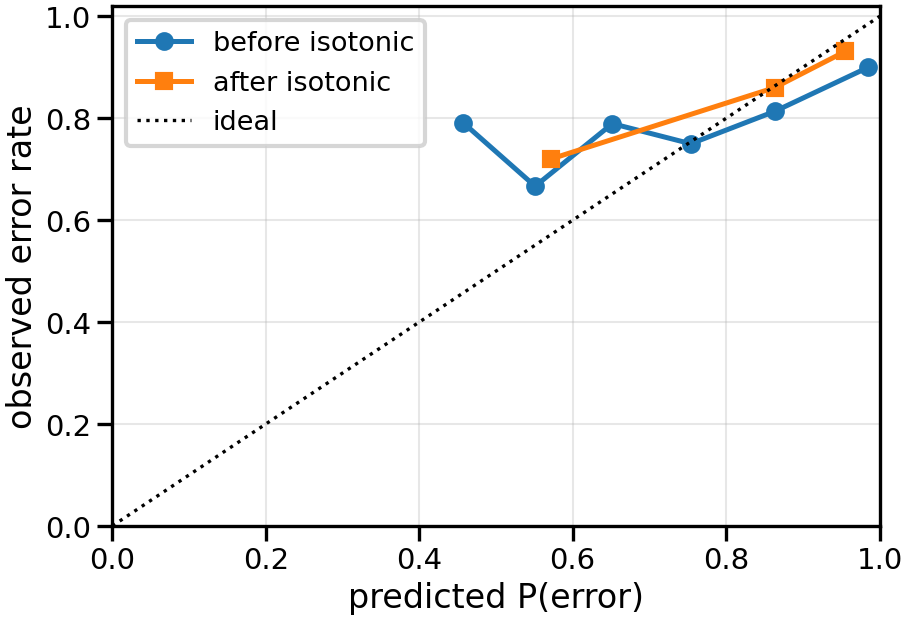
\includegraphics[width=\columnwidth]{F4_calibration.png}
\caption{Reliability of the risk estimate before and after isotonic correction.
Expected calibration error falls from 0.0895 to 0.0120.}
\label{fig:cal}
\end{figure}

\subsection{Which family is responsible}
Table~\ref{tab:abl} reports the ablation. Withholding retrieval costs roughly four
times what withholding the reader family costs, and withholding all five reader
signals yields an interval that spans zero.

\begin{table*}[!t]
\renewcommand{\arraystretch}{1.2}
\caption{Family-withholding ablation. $\Delta$AURC is measured against the full
sixteen-signal model; positive values indicate that removal degraded performance.}
\label{tab:abl}
\centering\footnotesize
\begin{tabular}{L{3.2cm}C{1.4cm}C{1.9cm}C{1.4cm}C{2.3cm}C{2.5cm}C{1.9cm}}
\toprule
\textbf{Configuration} & \textbf{Signals} & \textbf{Error AUC} & \textbf{AURC} &
\textbf{$\Delta$AURC vs full} & \textbf{95\% interval} & \textbf{Excludes zero} \\
\midrule
Full (R+D+A)   & 16 & 0.6390 & 0.8423 & ---              & ---                & --- \\
$-$ Retrieval  &  9 & 0.5410 & 0.8698 & \textbf{$+$0.0274} & 0.0149--0.0411   & yes \\
$-$ Agreement  & 12 & 0.6021 & 0.8513 & \textbf{$+$0.0103} & 0.0043--0.0173   & yes \\
$-$ Reader     & 11 & 0.6202 & 0.8467 & $+$0.0067          & $-0.0044$--0.0189 & \textbf{no} \\
Retrieval only &  7 & 0.5662 & 0.8640 & $+$0.0222          & 0.0088--0.0352   & yes \\
Agreement only &  4 & 0.5680 & 0.8694 & $+$0.0283          & 0.0138--0.0420   & yes \\
Reader only    &  5 & 0.5242 & 0.8785 & $+$0.0345          & 0.0191--0.0495   & yes \\
\bottomrule
\end{tabular}
\end{table*}

Permutation importance over the full model points the same way. The most
load-bearing signals are query--paragraph lexical overlap (retrieval, $\Delta$AURC
0.0121 when permuted), recurrence of the span in the second paragraph (agreement,
0.0107), span length (reader, 0.0103), span probability (reader, 0.0078) and best
fused score (retrieval, 0.0066). The reader's dedicated no-answer signal registers
$-0.0017$, indistinguishable from noise.

A caveat applies to any ablation over correlated inputs: because the families
encode overlapping information, withholding one bounds its contribution from below
rather than partitioning credit exactly. That two attribution methods agree
strengthens the reading without making it exact.

\section{Error Analysis and Transfer}
\begin{table}[!t]
\renewcommand{\arraystretch}{1.15}
\caption{Outcome taxonomy over all 3{,}585 test queries.}
\label{tab:tax}
\centering\footnotesize
\begin{tabular}{L{4.7cm}C{1.15cm}C{1.35cm}}
\toprule
\textbf{Outcome} & \textbf{Count} & \textbf{Share} \\
\midrule
Wrong span (source paragraph retrieved) & 1{,}844 & 51.4\,\% \\
Unanswerable query answered anyway      & 1{,}056 & 29.5\,\% \\
Correct                                 &    410 & 11.4\,\% \\
Retrieval failure (source not in top-$k$) & 219 &  6.1\,\% \\
Partial overlap below cut-off           &     56 &  1.6\,\% \\
\bottomrule
\end{tabular}
\end{table}

Span selection, not retrieval, dominates the failures (Table~\ref{tab:tax}). The
source paragraph enters the top five for 89.1\% of queries, after which the reader
selects a non-overlapping span in more than half of all cases; only 6.1\% fail
because retrieval missed. \textbf{The reader, not the retriever, is the bottleneck.}

Outcomes vary with interrogative type. Constrained answer forms fare best ---
\emph{when} 18.8\% ($n{=}256$), \emph{how many} 18.7\% ($n{=}257$), \emph{who}
16.1\% ($n{=}366$) --- because the span descriptors encode numerals and
capitalisation. Open forms fare worst: \emph{what} 8.9\% ($n{=}1{,}713$),
\emph{why} 1.7\% ($n{=}59$).

Three cases drawn verbatim from the test partition illustrate the behaviour. Asked
how many passengers passed through Bras\'ilia's airport in 2007, the reader returned
\textbf{11,119} where the reference is \textbf{11,119,872}; the truncated numeral
scores below cut-off and the risk estimate assigned it the highest value in the
partition, which is the correct decision. Asked for the fourth stomach compartment
in ruminants, it returned \textbf{abomasum} against \textbf{The abomasum} --- correct
after normalisation, and assigned the lowest risk. For the unanswerable query about
who appointed the governor of the Federal District before 1988, it returned
\textbf{Brazilian Federal Senate} at low risk: an entity of the expected type sitting
in a high-overlap sentence defeats every signal we compute, and this is precisely
the failure the agreement family was meant to catch and does not.

\begin{table*}[!t]
\renewcommand{\arraystretch}{1.2}
\caption{Reliability estimator fitted on Collection~A and evaluated on
Collection~B, whose articles are disjoint. ECE: expected calibration error.}
\label{tab:transfer}
\centering\footnotesize
\begin{tabular}{C{1.4cm}L{4.2cm}C{1.2cm}C{1.8cm}C{1.5cm}C{1.4cm}C{2.2cm}}
\toprule
\textbf{Procedure} & \textbf{Setting} & \textbf{$n$} & \textbf{Error AUC} &
\textbf{AURC} & \textbf{ECE} & \textbf{Base error rate} \\
\midrule
P1 & A $\rightarrow$ A within-collection & 3{,}585 & 0.6390 & 0.8423 & 0.0120 & 0.8856 \\
\textbf{P1} & \textbf{A $\rightarrow$ B transfer} & \textbf{1{,}000} & \textbf{0.6494} & 0.8612 & 0.0143 & 0.9000 \\
P1 & B $\rightarrow$ B within-collection & 1{,}000 & 0.5680 & 0.8843 & 0.0479 & 0.9000 \\
B5 & A $\rightarrow$ A within-collection & 3{,}585 & 0.5242 & 0.8785 & 0.0134 & 0.8856 \\
B5 & A $\rightarrow$ B transfer          & 1{,}000 & 0.5177 & 0.9003 & 0.0029 & 0.9000 \\
B5 & B $\rightarrow$ B within-collection & 1{,}000 & 0.5862 & 0.8773 & 0.0527 & 0.9000 \\
\bottomrule
\end{tabular}
\end{table*}

Across collections the P1 point estimate shows no large degradation (0.6494 against
0.6390 within-collection). We did not run a paired test across collections and
therefore do not assert that degradation is absent, only that the point estimate
does not display it. B5 does not transfer comparably (0.5177). P1 fitted on A also
exceeds P1 fitted on B itself (0.6494 against 0.5680), which we read as a
sample-size effect --- A supplies 2{,}400 reliability-training queries against B's
700 --- rather than any benefit of transfer. The setting shifts collection and
reader instance together and does not separate the two.

\section{Cost}
\begin{table}[!t]
\renewcommand{\arraystretch}{1.15}
\caption{Per-query cost, single CPU, $n=7{,}185$ queries; gate timed over 100
repetitions.}
\label{tab:lat}
\centering\footnotesize
\begin{tabular}{L{4.3cm}C{1.45cm}C{1.35cm}}
\toprule
\textbf{Stage} & \textbf{Median (ms)} & \textbf{p95 (ms)} \\
\midrule
Retrieval                     & 43.54 & 60.99 \\
Reader                        & 19.83 & 23.80 \\
Reliability signals           &  0.22 &  0.32 \\
Risk model $+$ gate           &  1.74 &  2.06 \\
\midrule
\textbf{End-to-end query}     & \textbf{63.77} & \textbf{83.03} \\
\textbf{Reliability layer}    & \textbf{1.96}  & \textbf{2.37} \\
\bottomrule
\end{tabular}
\end{table}

The reliability layer takes 1.96\,ms, near 3\% of a 63.77\,ms query, so criterion G6
is met with two orders of magnitude to spare (Table~\ref{tab:lat}). Retrieval
dominates. Peak resident memory reached 210.3\,MB, index construction over 5{,}637
paragraphs took 4.64\,s, and reader fitting 29.2\,s. Stored artefacts total
58.4\,MB. Nothing contacts the network at query time. These figures describe
\emph{this} system; they are small chiefly because no transformer is present, and
should not be read as a statement about a transformer pipeline.

Of seven pre-registered criteria, four were met (G0 control 0.4887; G3
$\Delta$AURC $-0.0345$; G4 $\Delta$AURC $-0.0293$; G6 layer 1.96\,ms) and three
were not: base reader accuracy 0.1144 against a 0.45 requirement (G1), a best
error-prediction ROC-AUC of 0.6390 against a 0.70 requirement (G2), and the
operating point of Section~\ref{sec:calib} (G5).

\section{Limitations}\label{sec:lim}
\textbf{The reader bounds every result.} Absent pretrained weights, the reader is a
classical feature-based span scorer. Base accuracy is 0.1144 and mean answer F1 is
0.145, so G1 fails by a wide margin and every finding is conditional on this reader.
A no-answer head trained on 130{,}319 queries rather than our 4{,}736 might carry
considerably more independent signal, which would raise the reader family's relative
contribution and narrow our conclusion to weak-reader regimes. Repeating the
measurement with a transformer reader is the most consequential outstanding step,
and the implementation is backend-agnostic to permit it.

\textbf{Error prediction is modest.} G2 fails; the best value is 0.6390. The estimate
orders queries better than chance and is useful for ranking, but is not strong
discrimination.

\textbf{No accuracy guarantee.} G5 fails and every procedure sits at zero coverage
for the 80\% target. Calibration succeeded in the score-to-frequency sense and
failed in the operating-point sense.

\textbf{Residual label risk.} After sibling masking, 2.39\% of substantive
unanswerable queries retain a plausible-answer string somewhere in the collection.
The string test is a proxy: presence does not establish answerability, and
paraphrase could make a query answerable with no string match.

\textbf{Adversarial construction.} SQuAD 2.0's unanswerable queries were written to
look plausible, and may be systematically easier or harder to detect than those
arising naturally. This dataset cannot resolve the question.

\textbf{Collection, language, granularity, scale.} English Wikipedia only, with no
technical, multilingual or specialist evaluation. Paragraph-level retrieval sidesteps
a segmentation confound but leaves the results inapplicable to systems that must
divide long documents. A single CPU with an exact index over 5{,}637 paragraphs
gives no evidence about million-paragraph collections under approximate search.

\textbf{Transfer and attribution.} One transfer setting, moving collection and reader
instance together, without a paired test across collections. Withholding a family of
correlated signals bounds its contribution from below rather than partitioning credit.

\textbf{No deployment evidence.} No user study, no field trial, no production data.
The system is a research prototype operating over a fixed collection; it is not
claimed to be production-ready, and no comparison to any commercial system is made
or implied.

\section{Conclusion}
We measured how much error-prediction information retrieval-side and cross-evidence
signals add beyond a reader-only calibrator in a CPU-only extractive
question-answering pipeline. Over 3{,}585 withheld SQuAD 2.0 queries from 36 unseen
articles, with article-level partitions and a passing shuffled-label control, the
combined representation raised error-prediction ROC-AUC from 0.5242 to 0.6390 and
lowered AURC by 0.0345 with a paired-bootstrap interval excluding zero. The ordering
persisted at three correctness cut-offs and under transfer to a disjoint collection,
and the layer cost 1.96\,ms of a 63.77\,ms query. Ablation and permutation importance
both attribute the contribution primarily to retrieval signals and secondarily to
agreement, with the reader family's independent contribution spanning zero.

Absolute quality is weak. Base reader accuracy is 0.1144, no procedure reached the
pre-registered error-prediction target, the intended 80\% operating point is
unreachable at any useful coverage, and three of seven criteria failed. We report the
incremental finding because it was measured, held under several analysis choices and
is inexpensive to adopt; we report the failures because a stronger reader could
change them, and because a reader unaware of them would be misled.

\section*{Acknowledgment}
The authors thank the Department of Computer Science and Engineering, AMC
Engineering College, for institutional support. SQuAD 2.0 is used under the terms
published by its authors.

\IEEEtriggeratref{7}
\begin{thebibliography}{99}
\footnotesize
\bibitem{kamath2020} A. Kamath, R. Jia, and P. Liang, ``Selective question
answering under domain shift,'' in \emph{Proc. 58th Annu. Meeting Assoc. Comput.
Linguistics (ACL)}, Jul. 2020, pp. 5684--5696, doi: 10.18653/v1/2020.acl-main.503.

\bibitem{rajpurkar2018} P. Rajpurkar, R. Jia, and P. Liang, ``Know what you don't
know: Unanswerable questions for SQuAD,'' in \emph{Proc. 56th Annu. Meeting Assoc.
Comput. Linguistics (ACL), Vol.~2: Short Papers}, Melbourne, Australia, Jul. 2018,
pp. 784--789, doi: 10.18653/v1/P18-2124.

\bibitem{dhuliawala2022} S. Dhuliawala, L. Adolphs, R. Das, and M. Sachan,
``Calibration of machine reading systems at scale,'' in \emph{Findings Assoc.
Comput. Linguistics: ACL 2022}, Dublin, Ireland, May 2022, pp. 1682--1693,
doi: 10.18653/v1/2022.findings-acl.133.

\bibitem{joren2025} H. Joren, J. Zhang, C.-S. Ferng, D.-C. Juan, A. Taly, and
C. Rashtchian, ``Sufficient context: A new lens on retrieval augmented generation
systems,'' in \emph{Proc. Int. Conf. Learn. Representations (ICLR)}, 2025.
[Online]. Available: https://arxiv.org/abs/2411.06037

\bibitem{abdumalikov2024} R. Abdumalikov, P. Minervini, and Y. Kementchedjhieva,
``Answerability in retrieval-augmented open-domain question answering,''
arXiv:2403.01461, Mar. 2024. [Online]. Available: https://arxiv.org/abs/2403.01461

\bibitem{muhamed2025} A. Muhamed, L. F. R. Ribeiro, M. Dreyer, V. Smith, and
M. T. Diab, ``RefusalBench: Generative evaluation of selective refusal in grounded
language models,'' arXiv:2510.10390, Oct. 2025. [Online]. Available:
https://arxiv.org/abs/2510.10390

\bibitem{lewis2021} P. Lewis, Y. Wu, L. Liu, P. Minervini, H. K\"uttler,
A. Piktus, P. Stenetorp, and S. Riedel, ``PAQ: 65 million probably-asked questions
and what you can do with them,'' \emph{Trans. Assoc. Comput. Linguistics}, vol.~9,
pp. 1098--1115, 2021, doi: 10.1162/tacl\_a\_00415.

\bibitem{elyaniv2010} R. El-Yaniv and Y. Wiener, ``On the foundations of
noise-free selective classification,'' \emph{J. Mach. Learn. Res.}, vol.~11,
pp. 1605--1641, May 2010.

\bibitem{geifman2017} Y. Geifman and R. El-Yaniv, ``Selective classification for
deep neural networks,'' in \emph{Adv. Neural Inf. Process. Syst. (NeurIPS)}, Long
Beach, CA, USA, 2017, pp. 4878--4887.

\bibitem{guo2017} C. Guo, G. Pleiss, Y. Sun, and K. Q. Weinberger, ``On
calibration of modern neural networks,'' in \emph{Proc. 34th Int. Conf. Mach.
Learn. (ICML)}, PMLR vol.~70, Sydney, Australia, 2017, pp. 1321--1330.

\bibitem{zadrozny2002} B. Zadrozny and C. Elkan, ``Transforming classifier scores
into accurate multiclass probability estimates,'' in \emph{Proc. 8th ACM SIGKDD
Int. Conf. Knowl. Discovery Data Mining (KDD)}, Edmonton, Canada, 2002,
pp. 694--699, doi: 10.1145/775047.775151.

\bibitem{deerwester1990} S. Deerwester, S. T. Dumais, G. W. Furnas, T. K.
Landauer, and R. Harshman, ``Indexing by latent semantic analysis,'' \emph{J.
Amer. Soc. Inf. Sci.}, vol.~41, no.~6, pp. 391--407, Sep. 1990.

\bibitem{robertson2009} S. Robertson and H. Zaragoza, ``The probabilistic
relevance framework: BM25 and beyond,'' \emph{Found. Trends Inf. Retrieval},
vol.~3, no.~4, pp. 333--389, 2009, doi: 10.1561/1500000019.
\end{thebibliography}

\end{document}
